\section{Sjenčanje (shading)}

\begin{figure}[H]
\caption{Model osjenčan difuznom rasvjetom}
\label{fig:monkey-plastic}
\begin{center}
\fbox{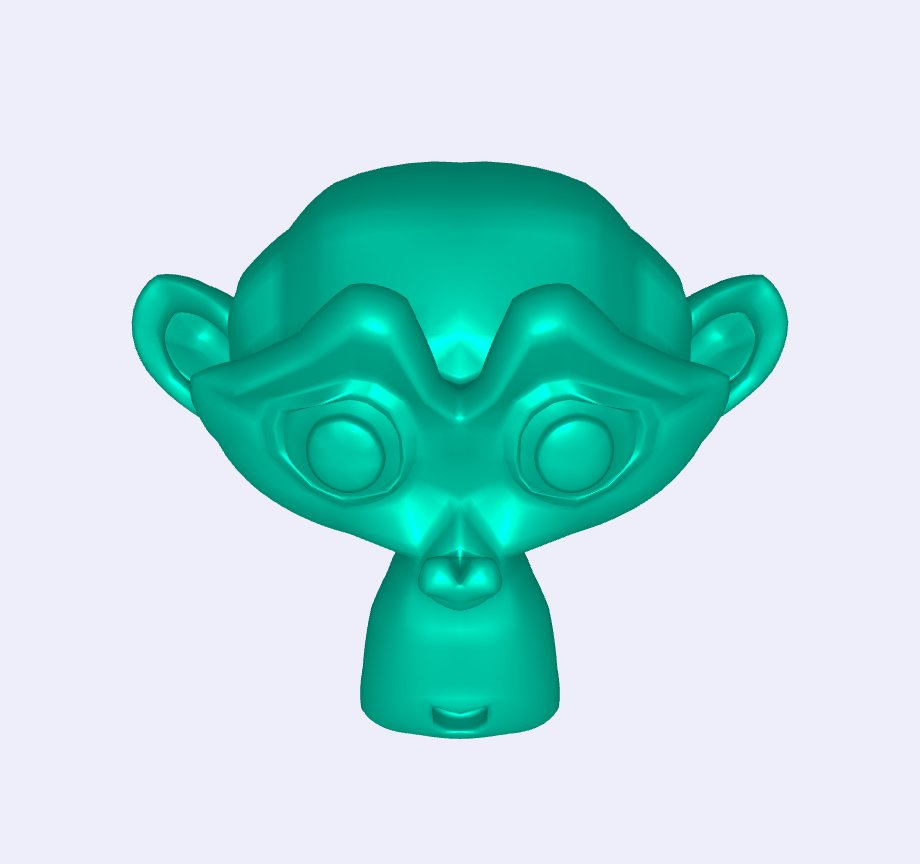
\includegraphics[scale=0.3]{monkey_plastic.png}}
\end{center}
\end{figure}

\subsection{Cel-shading princip}

\begin{figure}[H]
\caption{Model osjenčan toon shaderom}
\label{fig:monkey-toonshaded}
\begin{center}
\fbox{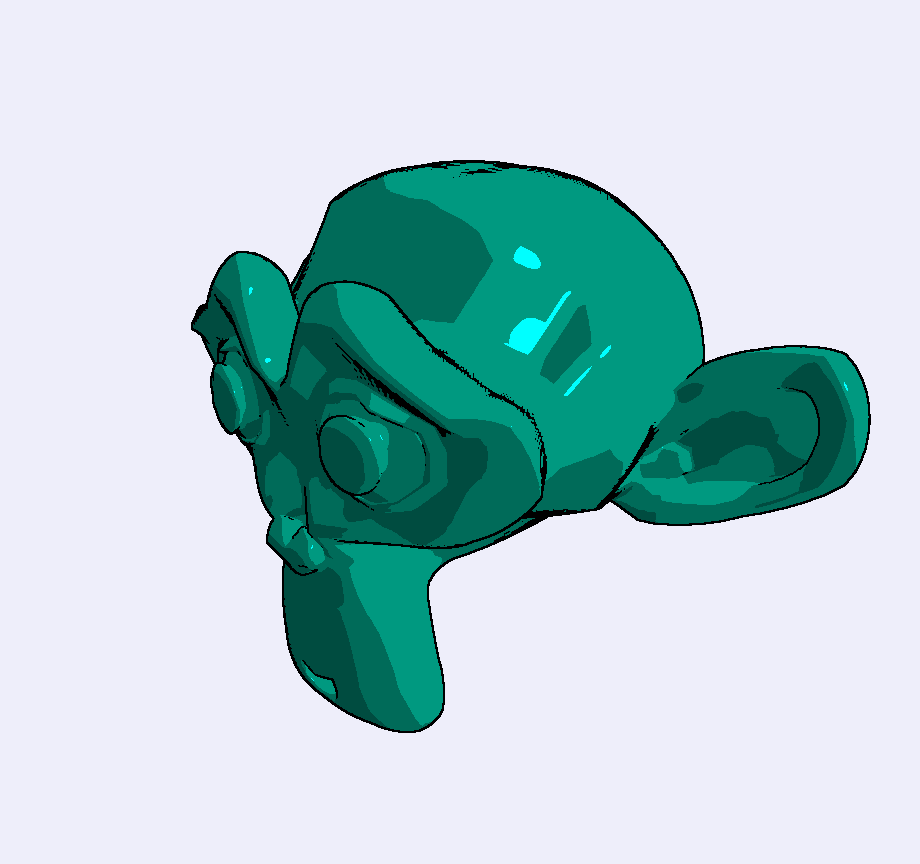
\includegraphics[scale=0.3]{monkey_toonshaded.png}}
\end{center}
\end{figure}

Što je to uopće i kako se postiže. Koji koraci(slojevi) su potrebni

\subsection{Iscrtavanje obrisa i rubova}

\begin{figure}[H]
\caption{Model s iscrtanom \emph{dubinom} pixel-a}
\label{fig:monkey-depth}
\begin{center}
\fbox{
\includegraphics[scale=0.3]{monkey_depth.png}}
\end{center}
\end{figure}


\begin{figure}[H]
\caption{Model s iscrtanim obrisima}
\label{fig:monkey-edges}
\begin{center}
\fbox{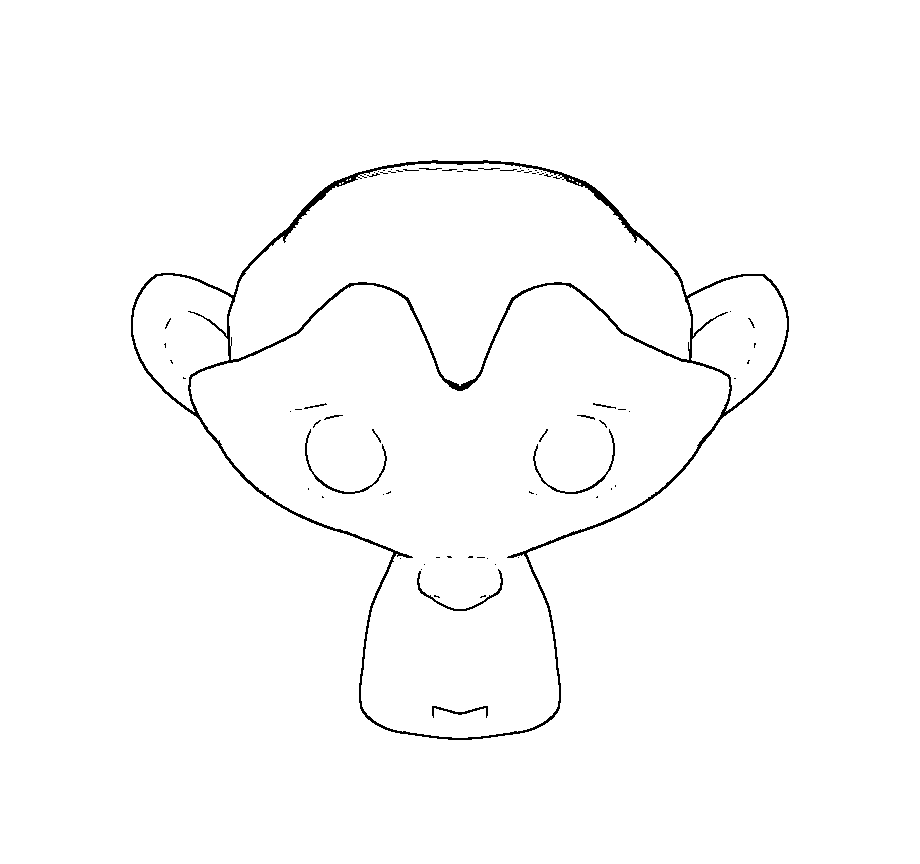
\includegraphics[scale=0.3]{monkey_edges.png}}
\end{center}
\end{figure}

\subsection{Sjenčanje}

\begin{figure}[H]
\caption{Osjenčani model}
\label{fig:monkey-toon}
\begin{center}
\fbox{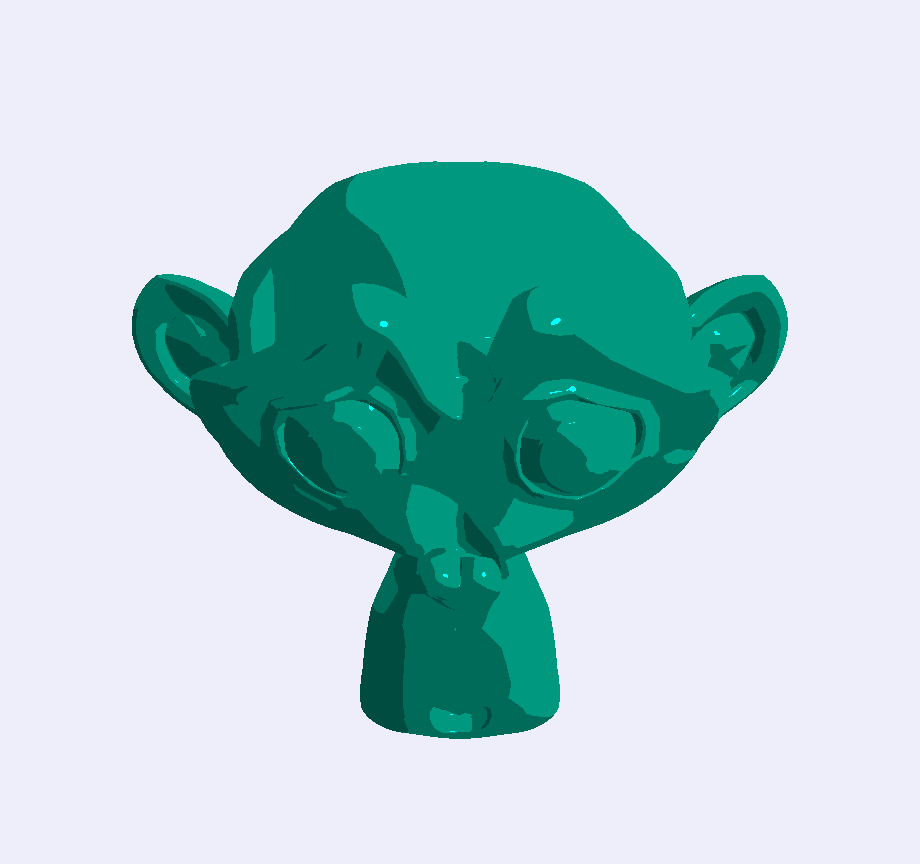
\includegraphics[scale=0.3]{monkey_toon.png}}
\end{center}
\end{figure}

\subsection{Spajanje slojeva}

\begin{figure}[H]
\caption{Rezultat dobiven spajanjem slojeva}
\label{fig:monkey-final}
\begin{center}
\fbox{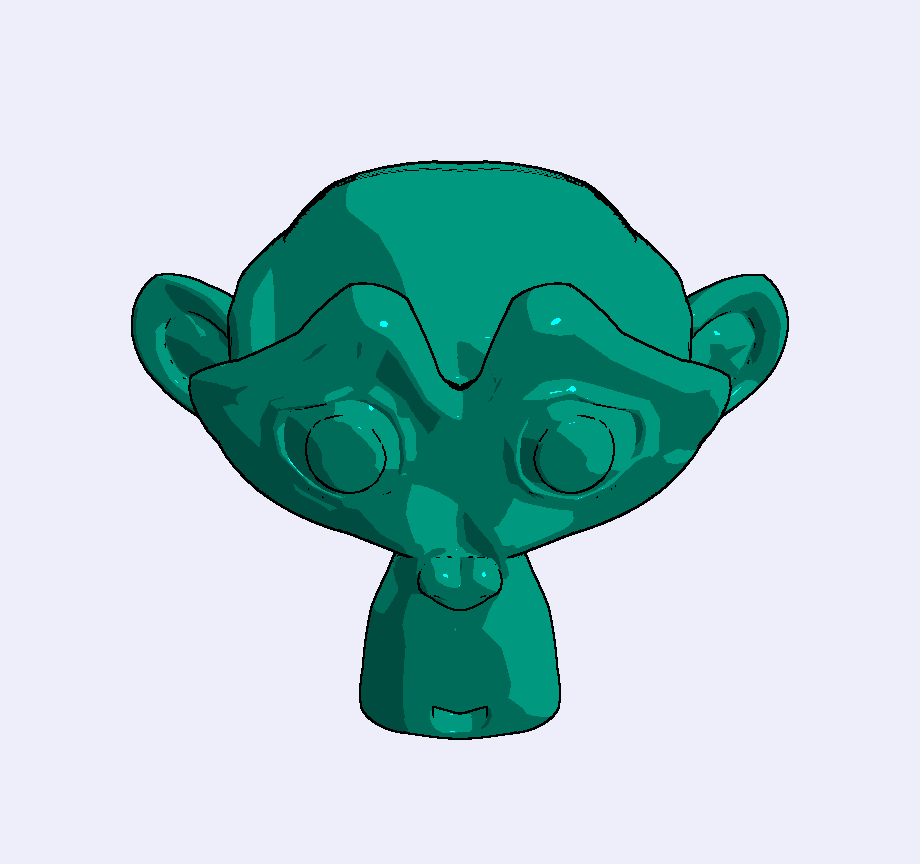
\includegraphics[scale=0.3]{monkey_final.png}}
\end{center}
\end{figure}

Kako se spajaju u cjelinu i što dobijemo s time. Spomenuti ograničenje WebGL-a ovdje